% !TeX root = ecn-encap-test_tr
% ================================================================
\section{History of ECN propagation by tunnels}\label{ecn-encap-test_History}

\begin{figure}[h]
	\centering
	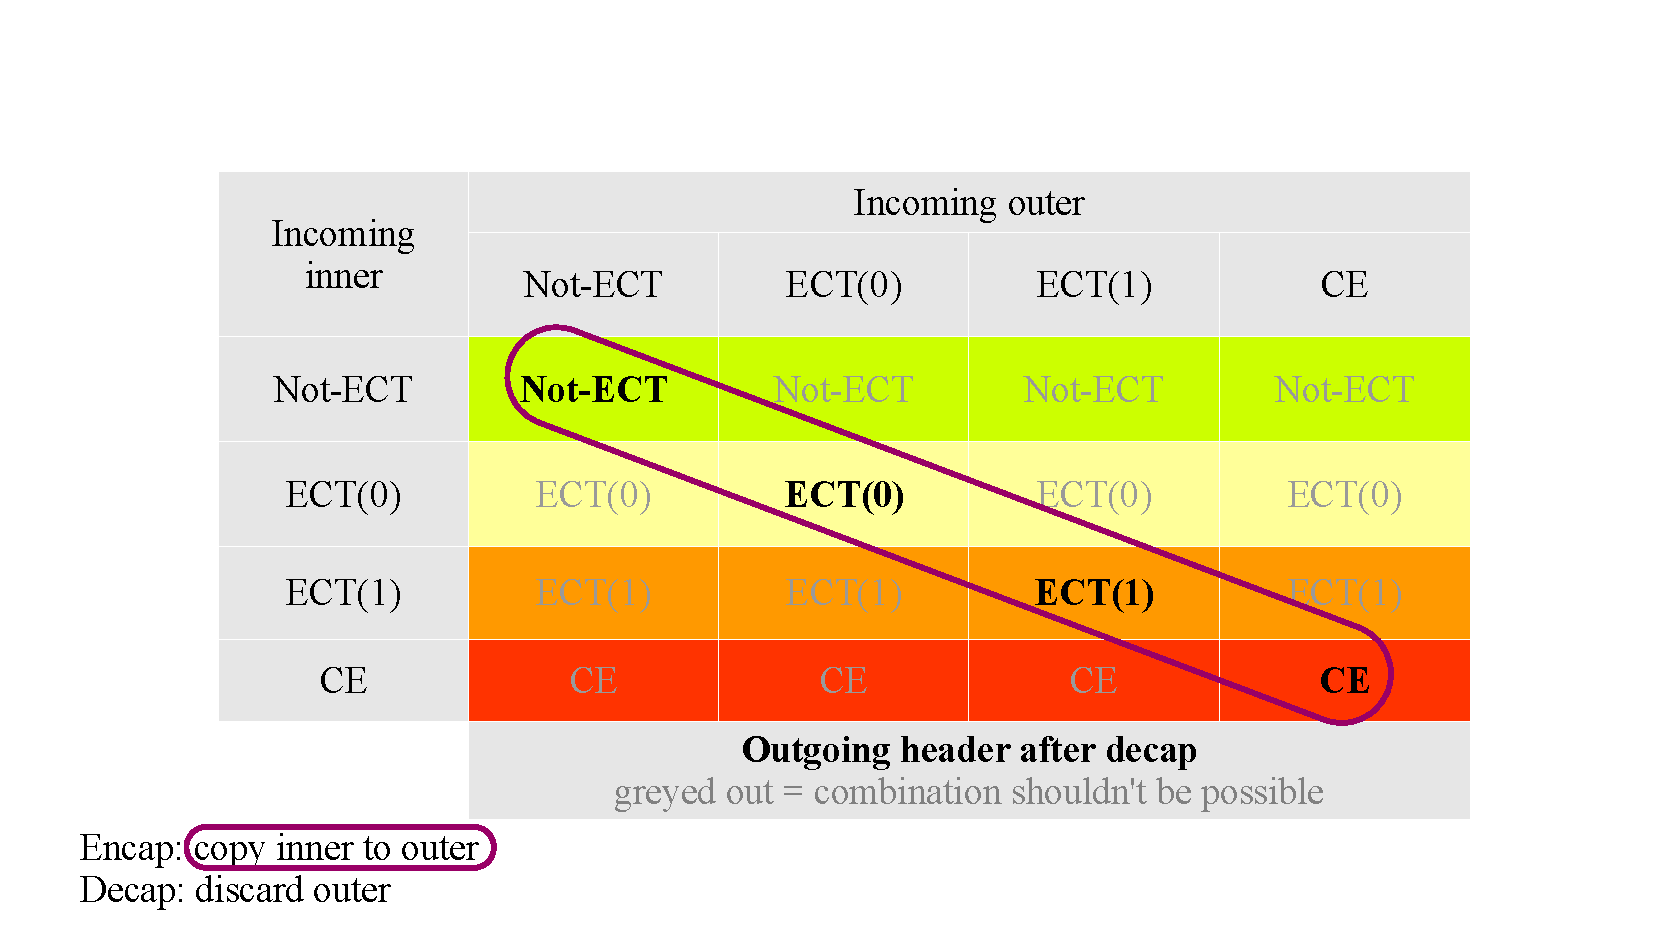
\includegraphics[width=\linewidth,clip]{ecn-tunnel-testing-bg-1}
	\caption{Simple (pre-ECN) tunnel, e.g.\ RFC2003}\label{fig:ecn-tunnel-testing-bg-1}
\end{figure}
\begin{figure}[h]
	\centering
	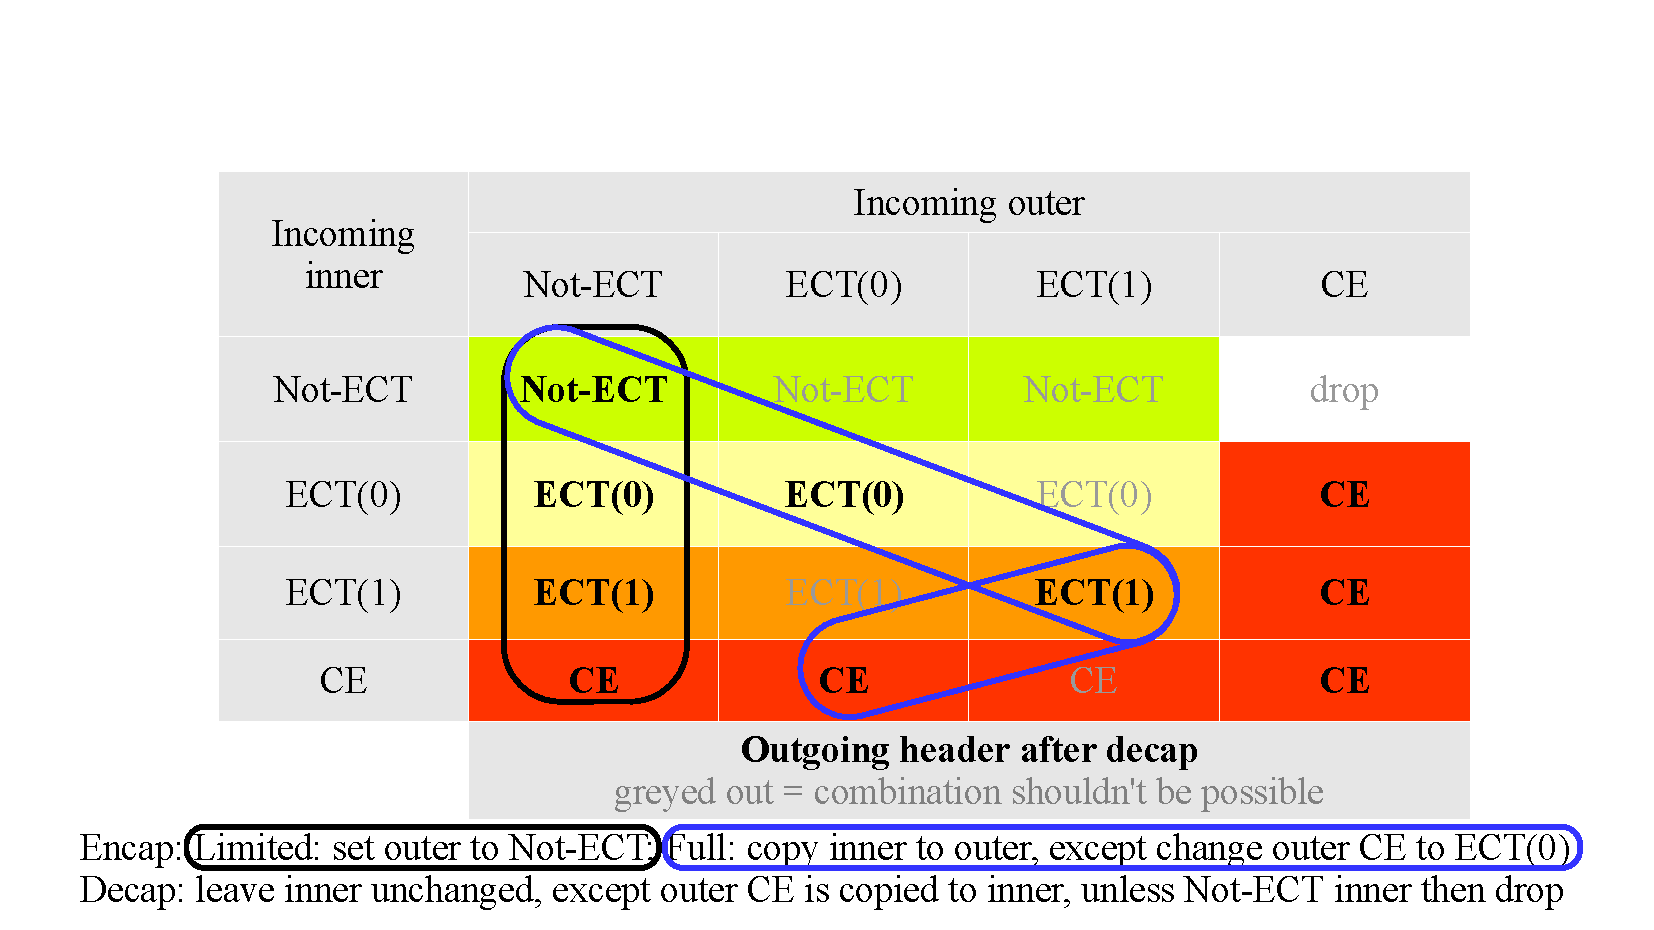
\includegraphics[width=\linewidth,clip]{ecn-tunnel-testing-bg-2}
	\caption{Original RFC~3168 ECN-tunnel~\cite{rfc3168}}\label{fig:ecn-tunnel-testing-bg-2}
\end{figure}

Figures \ref{fig:ecn-tunnel-testing-bg-1}--\ref{fig:ecn-tunnel-testing-bg-4} illustrate the evolution of ECN tunnelling, starting from pre-ECN days in \autoref{fig:ecn-tunnel-testing-bg-1}.

The table in each figure visualizes the outcome as each spec slightly altered the decapsulation rules. The rows represent the Inner and the columns represent the Outer header arriving at the tunnel egress. The text in each cell (and the associated background colour) gives the Onward (outgoing) header. 

The loops group together the combinations of Inner and Outer that would be expected, given the behaviour of an encapsulator that complies with the same spec as the decapsulator. Where the spec allows two encap options, different coloured loops are shown for each.

\newpage
\begin{figure}[h]
	\centering
	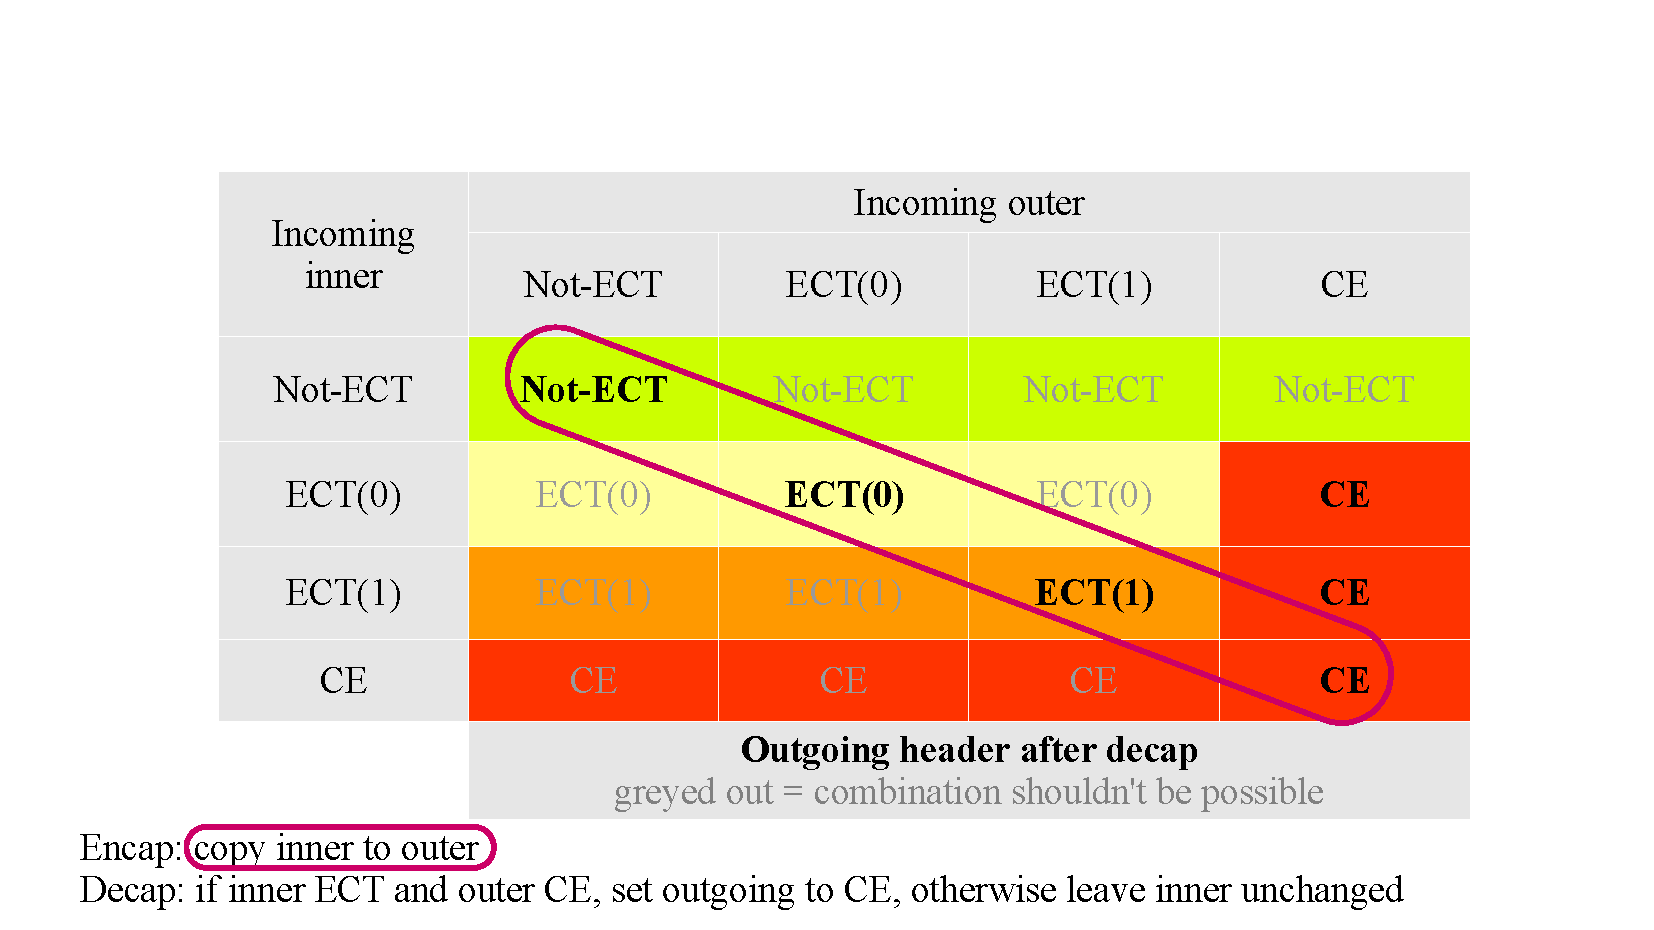
\includegraphics[width=\linewidth,clip]{ecn-tunnel-testing-bg-3}
	\caption{IPsec v2 (RFC~4301)~\cite{IETF_RFC4301:IPSEC_architecture}}\label{fig:ecn-tunnel-testing-bg-3}
\end{figure}
\begin{figure}[h]
	\centering
	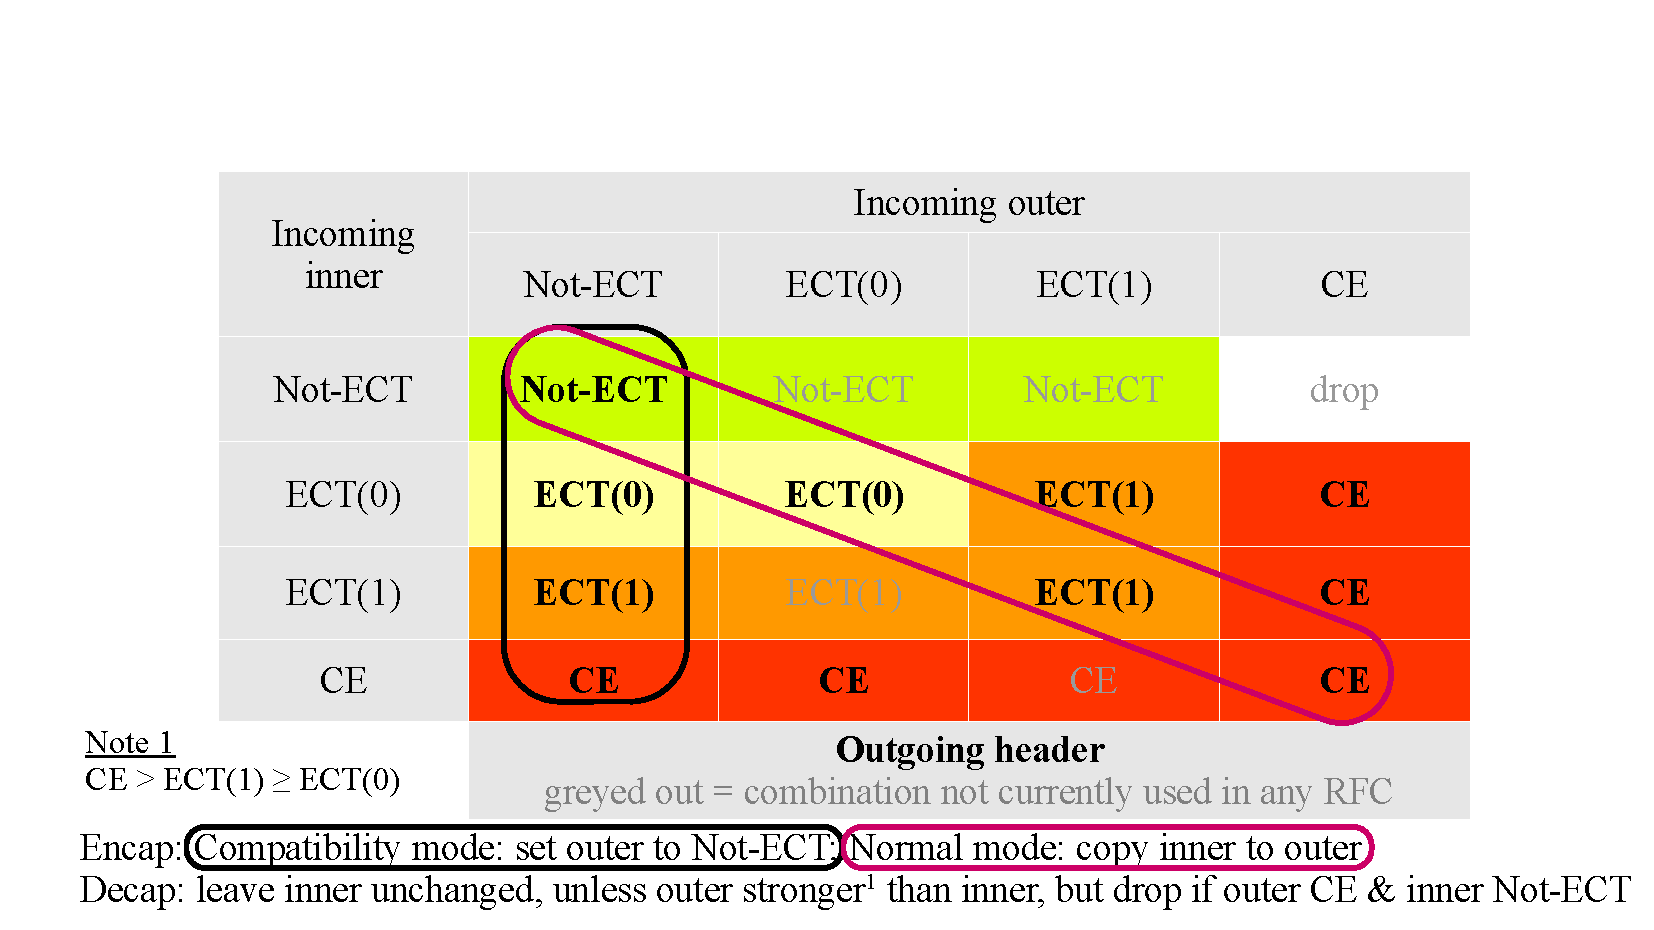
\includegraphics[width=\linewidth,clip]{ecn-tunnel-testing-bg-4}
	\caption{Universal ECN tunnel (RFC~6040)~\cite{Briscoe07b:ECN-tunnel}}\label{fig:ecn-tunnel-testing-bg-4}
\end{figure}

The text in cells outside the loops is greyed out to illustrate that this combination would not be expected. Nonetheless, some other combinations of Inner and Outer can occur when an encap complying with one spec is paired with a decap complying with another. \autoref{fig:ecn-tunnel-testing-bg-5} overlays the three behaviours that correctly propagate ECN to show how the three specs interact with each other. It shows the union of all three possible encap behaviours as not greyed out text, and two colours are used for the cell background where there are two possible decap behaviours.

\begin{figure}[h]
	\centering
	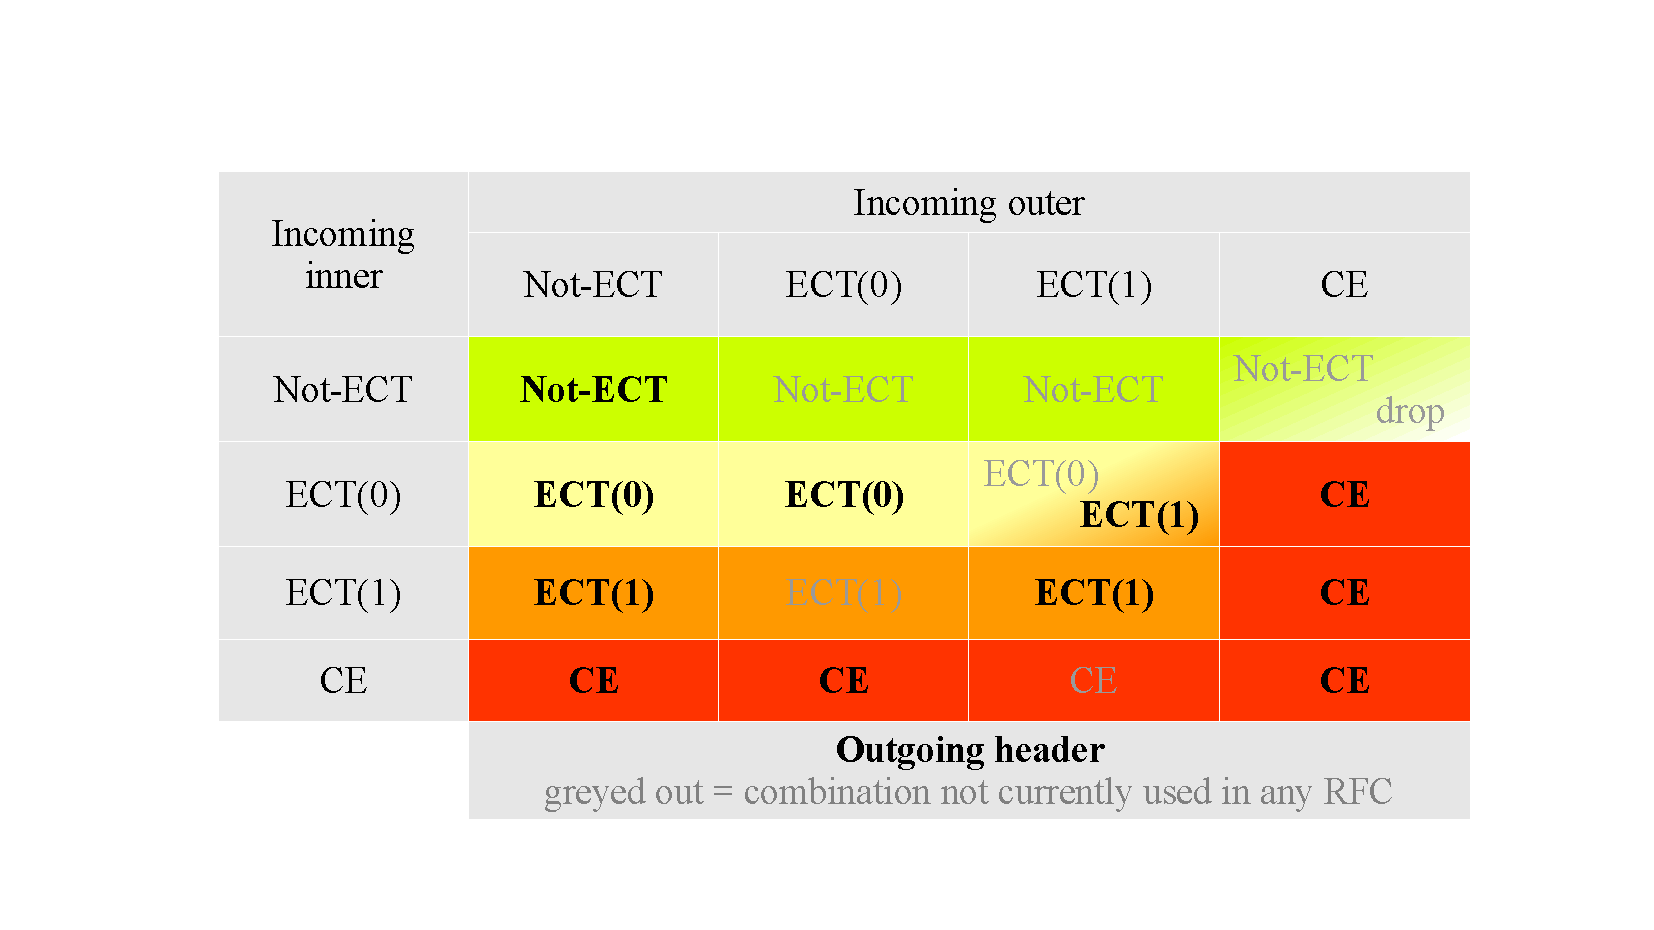
\includegraphics[width=\linewidth,clip]{ecn-tunnel-testing-bg-5}
	\caption{Black box view of all three combinations of ECN-tunnel specs (Figures \ref{fig:ecn-tunnel-testing-bg-2}--\ref{fig:ecn-tunnel-testing-bg-4})}\label{fig:ecn-tunnel-testing-bg-5}
\end{figure}





